\begin{figure*}[hbtp]
  \centering
  \subfigure[Initial graph]{
    \label{fig:about-df-01}
    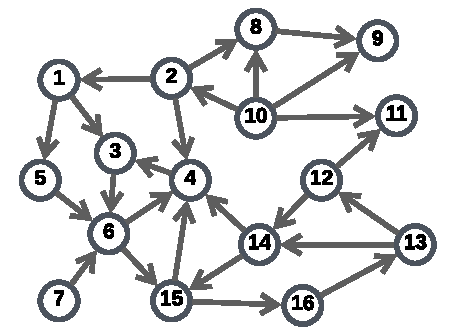
\includegraphics[width=0.23\linewidth]{out/about-df-01.pdf}
  }
  \subfigure[Marking affected (initial)]{
    \label{fig:about-df-02}
    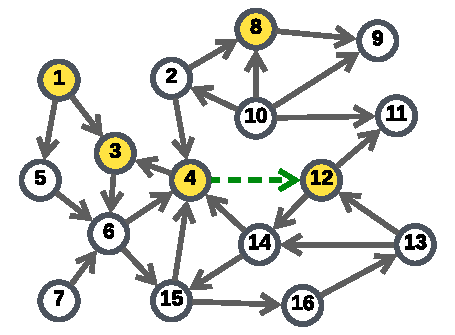
\includegraphics[width=0.23\linewidth]{out/about-df-02.pdf}
  }
  \subfigure[After first iteration]{
    \label{fig:about-df-03}
    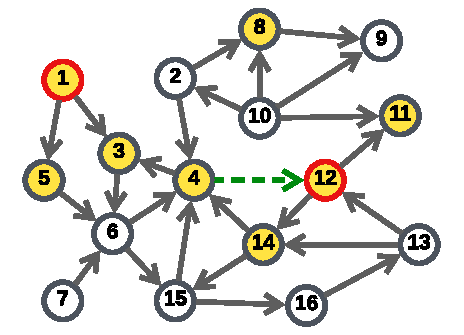
\includegraphics[width=0.23\linewidth]{out/about-df-03.pdf}
  }
  \subfigure[After second iteration]{
    \label{fig:about-df-04}
    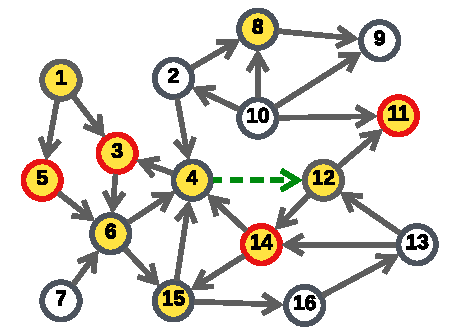
\includegraphics[width=0.23\linewidth]{out/about-df-04.pdf}
  } \\[-2ex]
  % \subfigure[]{
  %   \label{fig:about-df-05}
  %   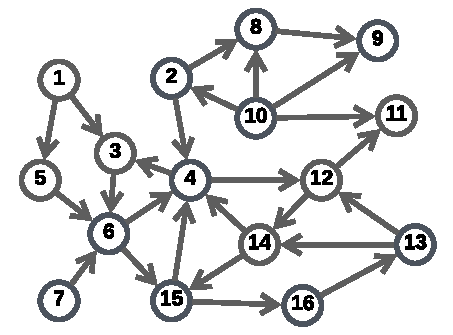
\includegraphics[width=0.18\linewidth]{out/about-df-05.pdf}
  % }
  \caption{An example explaining the \textit{Dynamic Frontier} approach. Affected vertices are shown with yellow fill, and vertices with a change in rank greater than frontier tolerance $\tau'$ are shown with red border.}
  \label{fig:about-df}
\end{figure*}




% \begin{figure*}[hbtp]
%   \centering
%   \subfigure{
%     \label{fig:about-dynamic-df-detail}
%     \includegraphics[width=0.84\linewidth]{out/about-dynamic-frontier.jpg}
%   } \\[-2ex]
%   \caption{Process of marking affected nodes. Figure (a) on the left is the graph $G^{t-1}$, Figure (b) shows the graph $G^t$ with two new edges, shown in dashed lines, added. Vertices filled in Figure (b) indicate the affected vertices. The numbers on the vertices in Figure (b) indicate the iteration at which the vertex is marked as affected.}
%   \label{fig:about-dynamic-frontier}
% \end{figure*}
